% Auto-generated by `python new.py summarize` on 2026-06-10T10:36:21.
% Folder: experiments/2026-06-10_u_axes_by_choice/
% Paste into a beamer document. Adjust the graphicspath or paths below if compiling from a different working directory.
%
% Requires: \usepackage{graphicx}

\begin{frame}{Qwen 0.5B — per-layer CKA(U,P\_U) and CKA(U,I) split by model choice}
  \begin{center}
    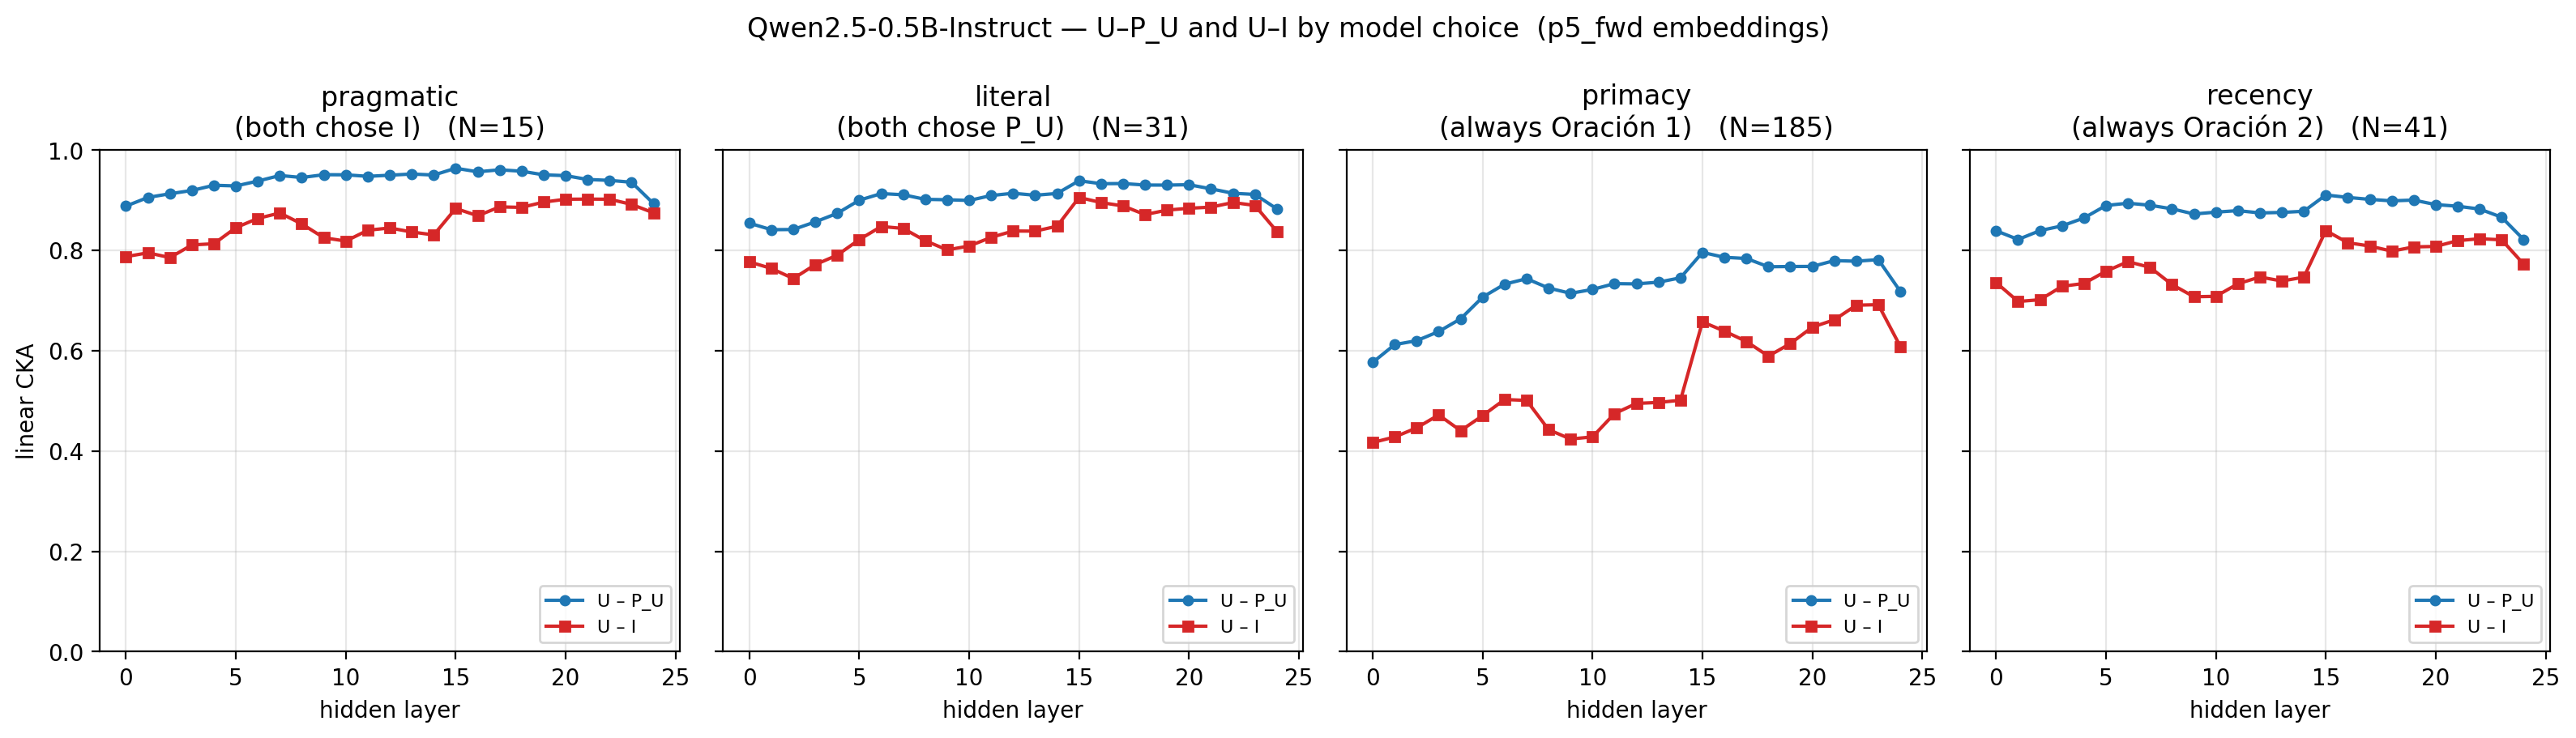
\includegraphics[width=0.95\textwidth,height=0.82\textheight,keepaspectratio]{experiments/2026-06-10_u_axes_by_choice/plots/Qwen2.5-0.5B-Instruct_curves.png}
  \end{center}
\end{frame}

\begin{frame}{Qwen 0.5B — per-layer CKA(U,P\_U) and CKA(U,I) split by model choice}
  \small
  \textbf{Computation.} Embeddings are taken from the p5_fwd run: $U=$ bracket\_answer, $P_U=$ bracket\_sentence\_1 (the S4 fill), $I=$ bracket\_sentence\_2 (the P fill). Each of the 272 stimuli is classified by the pair (fwd answer $a_f$, rev answer $a_r$) into one of 4 subsets: pragmatic ($a_f{=}1,a_r{=}0$ — chose $I$ in both directions, $N{=}15$), literal ($a_f{=}0,a_r{=}1$ — chose $P_U$ in both, $N{=}31$), primacy ($a_f{=}a_r{=}0$ — always Oración 1, $N{=}185$), recency ($a_f{=}a_r{=}1$ — always Oración 2, $N{=}41$). For each subset, restrict the per-row embeddings to its rows; for every hidden layer $L$ build centered Gram matrices $K_X[L]=X_c X_c^{\!\top}$ with $X_c=X-\bar X$ for $X\in\{U,P_U,I\}$; plot linear CKA $\langle K_U,K_X\rangle_F/(\|K_U\|_F\|K_X\|_F)$ for $X\in\{P_U,I\}$ vs $L$. One panel per subset, sharing the y-axis.
  \par\vspace{0.8em}
  \textbf{Interpretation.} Pragmatic and literal are content-decided subsets; primacy and recency are position-decided. If the choice tracks the internal representation, the pragmatic panel should show $U$–$I$ above $U$–$P_U$ (the model picked $I$ because $U$ aligned with it), and literal should show the inverse. Panel-independence (all four look the same) would mean the choice is decoupled from $U$'s alignment — i.e. the model's behaviour is driven by something other than the geometry we're probing. Caveat: $N{=}15$ and $N{=}31$ are tiny, so CKA estimates there have high variance and an upward bias; compare the within-panel $U$–$P_U$ vs $U$–$I$ gap, not the absolute heights across panels.
\end{frame}

\begin{frame}{Qwen 0.5B — layer×layer cross-bracket CKA split by model choice}
  \begin{center}
    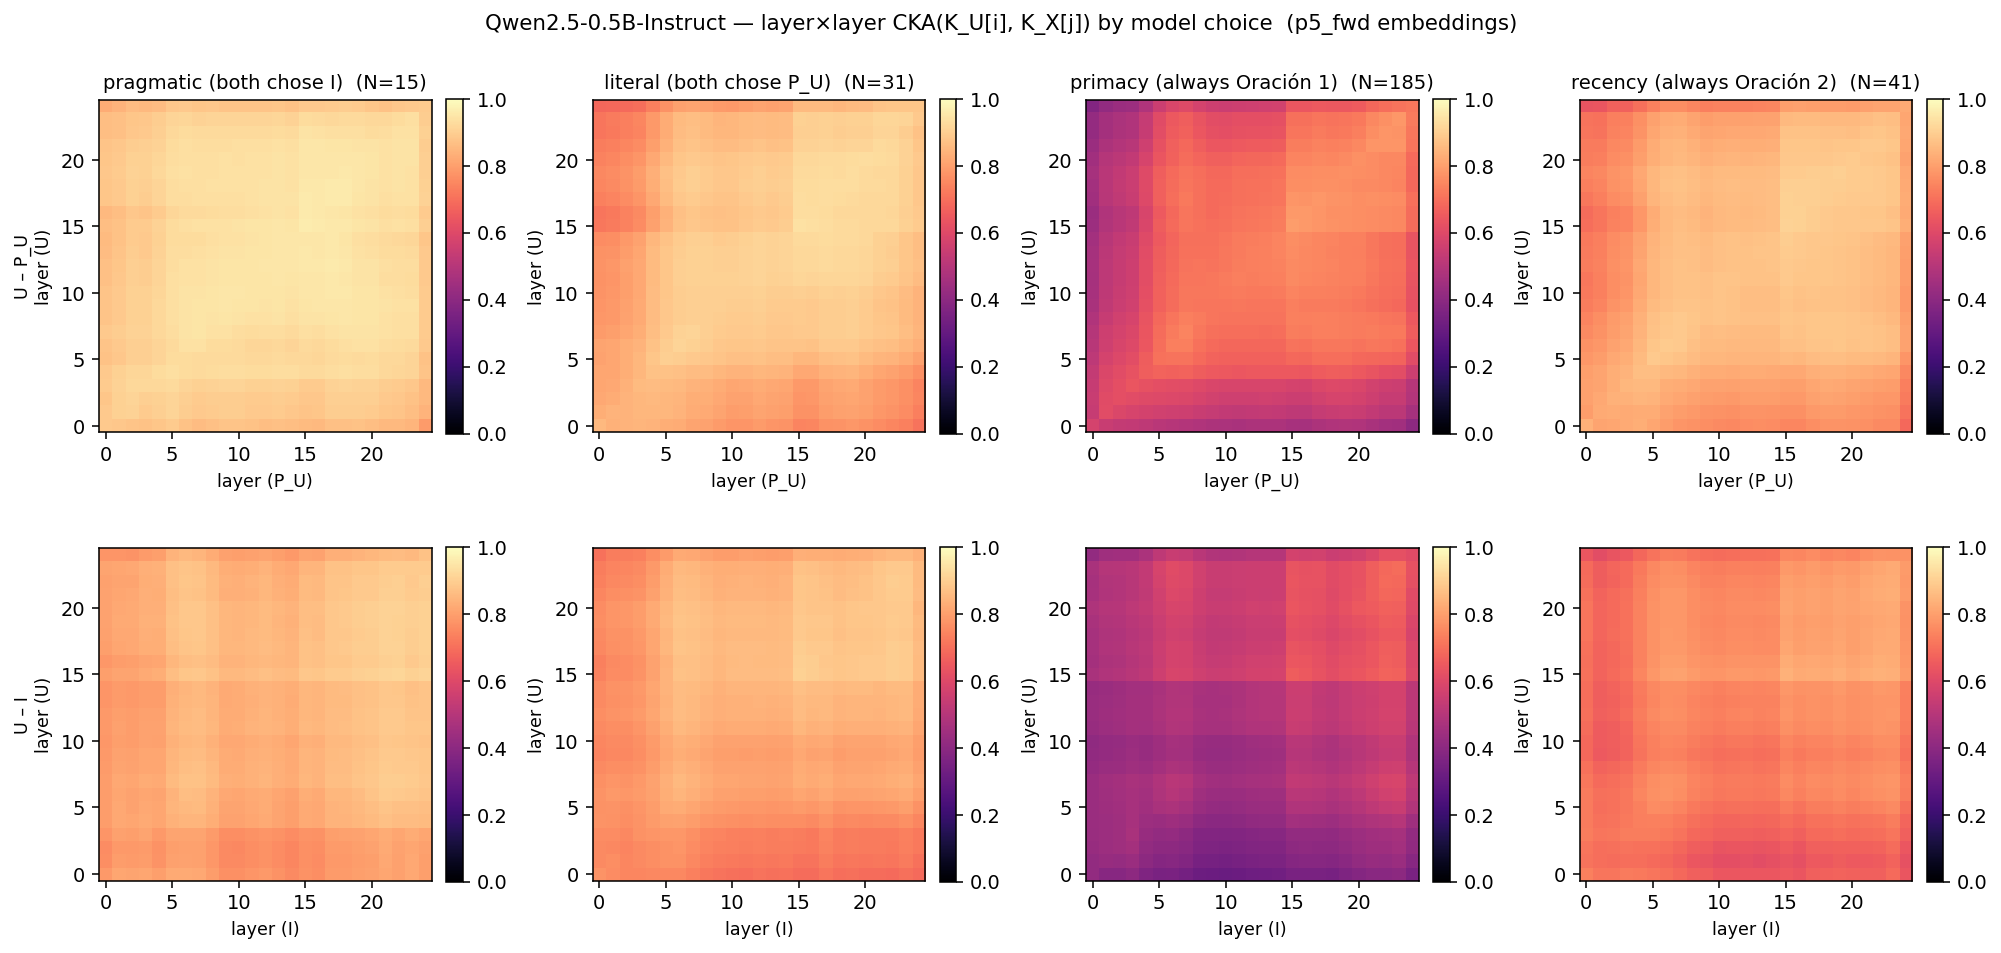
\includegraphics[width=0.95\textwidth,height=0.82\textheight,keepaspectratio]{experiments/2026-06-10_u_axes_by_choice/plots/Qwen2.5-0.5B-Instruct_layer_vs_layer.png}
  \end{center}
\end{frame}

\begin{frame}{Qwen 0.5B — layer×layer cross-bracket CKA split by model choice}
  \small
  \textbf{Computation.} Uses the same per-subset centered kernels as the curves plot. For each of the 4 subsets and each $X\in\{P_U,I\}$, build the $L\times L$ matrix $M_X[i,j]=\mathrm{CKA}(K_U[i],K_X[j])$. Grid: rows are the 4 subsets (pragmatic, literal, primacy, recency); columns are the pair (left $U$–$P_U$, right $U$–$I$). Diagonal cells $M_X[i,i]$ reproduce the per-layer curves from the other plot.
  \par\vspace{0.8em}
  \textbf{Interpretation.} Off-diagonal brightness means $U$'s geometry at layer $i$ already matches the other bracket's geometry at a different layer $j$ — a cross-depth (delayed or anticipated) binding. Reading down a column compares the same bracket-pair across choice subsets: if the pragmatic row's $U$–$I$ heatmap has earlier off-diagonal bleed than primacy's, the model's content-driven $I$ pick corresponds to an earlier internal binding. Position-driven rows (primacy, recency) are expected to look like the population baseline; deviation in the content rows is the signal. Small-N rows (pragmatic, literal) inflate CKA — read structure, not absolute brightness.
\end{frame}
